\begin{frame}{Exemple}
    \begin{center}
        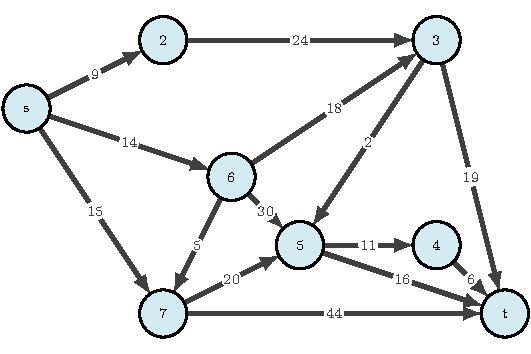
\includegraphics[height=.6\textheight]{fig/ordinal-0.pdf}

        Ordre topologique : $s,6,7,2,3,5,4,t$
    \end{center}
\end{frame}

\begin{frame}{Itérations de l'algorithme : traitement de $s$}
    \begin{center}
        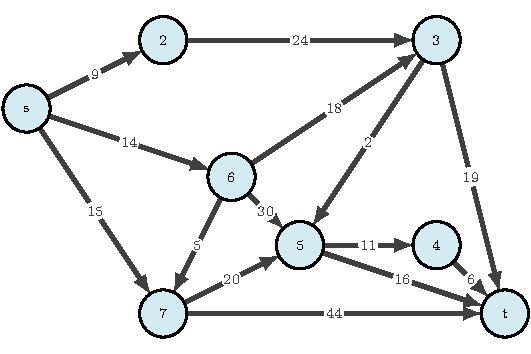
\includegraphics[height=.6\textheight]{fig/ordinal-0.pdf}      
    \begin{tabular}{c|cccccccc}
        
        sommet & s       &2      &7      &6      &5      &3      &4      &t      \\
        \hline
        \texttt{pred} & &       &       &       &       &       &       &       \\
        \texttt{dist} & 0       &$+\infty$    &$+\infty$    &$+\infty$    &$+\infty$    &$+\infty$    &$+\infty$    &$+\infty$    \\
    \end{tabular}
\end{center}
\end{frame}

\begin{frame}{Itérations de l'algorithme : traitement de $6$}
    \begin{center}
        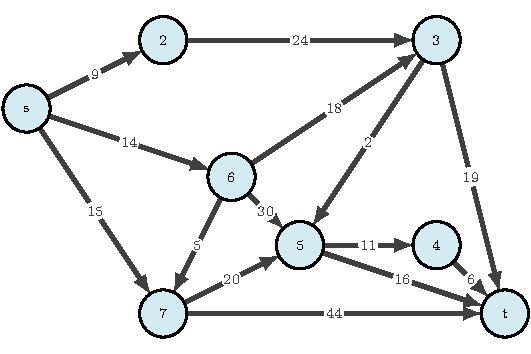
\includegraphics[height=.6\textheight]{fig/ordinal-0.pdf}      
    \begin{tabular}{c|cccccccc}
        
        sommet & s       &2      &7      &6      &5      &3      &4      &t      \\
        \hline
        \texttt{pred} & &       &       &s      &       &       &       &       \\
        \texttt{dist} & 0       &$+\infty$    &$+\infty$    &14     &$+\infty$    &$+\infty$    &$+\infty$    &$+\infty$    \\
    \end{tabular}
\end{center}
\end{frame}

\begin{frame}{Itérations de l'algorithme : traitement de $7$}
    \begin{center}
        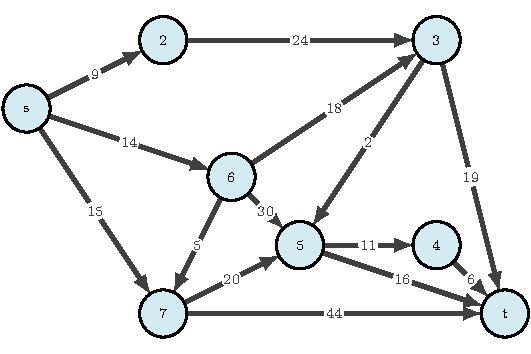
\includegraphics[height=.6\textheight]{fig/ordinal-0.pdf}      
    \begin{tabular}{c|cccccccc}
        
        sommet & s       &2      &7      &6      &5      &3      &4      &t      \\
        \hline
        \texttt{pred} & &       &s      &s      &       &       &       &       \\
        \texttt{dist} & 0       &$+\infty$    &15     &14     &$+\infty$    &$+\infty$    &$+\infty$    &$+\infty$    \\
    \end{tabular}
\end{center}
\end{frame}

\begin{frame}{Itérations de l'algorithme : traitement de $2$}
    \begin{center}
        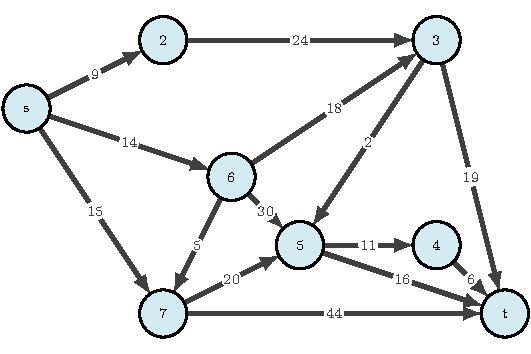
\includegraphics[height=.6\textheight]{fig/ordinal-0.pdf}      
    \begin{tabular}{c|cccccccc}
        
        sommet & s       &2      &7      &6      &5      &3      &4      &t      \\
        \hline
        \texttt{pred} & &s      &s      &s      &       &       &       &       \\
        \texttt{dist} & 0       &9      &15     &14     &$+\infty$    &$+\infty$    &$+\infty$    &$+\infty$    \\
    \end{tabular}
\end{center}
\end{frame}

\begin{frame}{Itérations de l'algorithme : traitement de $3$}
    \begin{center}
        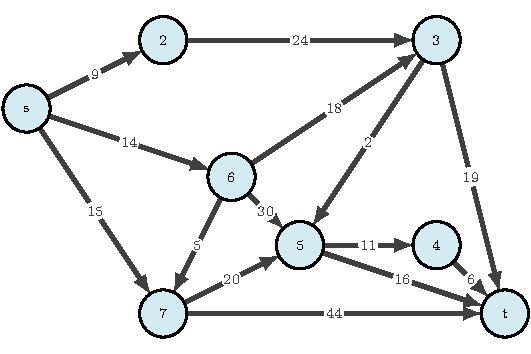
\includegraphics[height=.6\textheight]{fig/ordinal-0.pdf}      
    \begin{tabular}{c|cccccccc}
        
        sommet & s       &2      &7      &6      &5      &3      &4      &t      \\
        \hline
        \texttt{pred} & &s      &s      &s      &       &6      &       &       \\
        \texttt{dist} & 0       &9      &15     &14     &$+\infty$    &32     &$+\infty$    &$+\infty$    \\
    \end{tabular}
\end{center}
\end{frame}

\begin{frame}{Itérations de l'algorithme : traitement de $5$}
    \begin{center}
        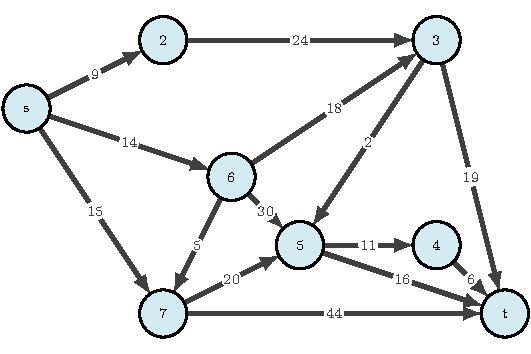
\includegraphics[height=.6\textheight]{fig/ordinal-0.pdf}      
    \begin{tabular}{c|cccccccc}
        
        sommet & s       &2      &7      &6      &5      &3      &4      &t      \\
        \hline
        \texttt{pred} & &s      &s      &s      &3      &6      &       &       \\
        \texttt{dist} & 0       &9      &15     &14     &34     &32     &$+\infty$    &$+\infty$    \\
    \end{tabular}
\end{center}
\end{frame}

\begin{frame}{Itérations de l'algorithme : traitement de $4$}
    \begin{center}
        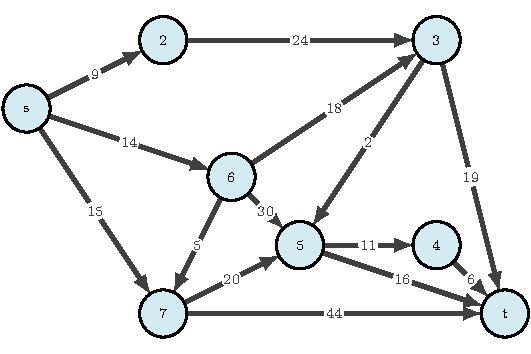
\includegraphics[height=.6\textheight]{fig/ordinal-0.pdf}      
    \begin{tabular}{c|cccccccc}
        
        sommet & s       &2      &7      &6      &5      &3      &4      &t      \\
        \hline
        \texttt{pred} & &s      &s      &s      &3      &6      &5      &       \\
        \texttt{dist} & 0       &9      &15     &14     &34     &32     &45     &$+\infty$    \\
    \end{tabular}
\end{center}
\end{frame}

\begin{frame}{Itérations de l'algorithme : traitement de $t$}
    \begin{center}
        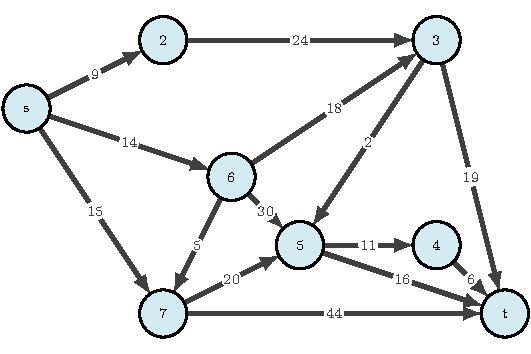
\includegraphics[height=.6\textheight]{fig/ordinal-0.pdf}      
    \begin{tabular}{c|cccccccc}
        
        sommet & s       &2      &7      &6      &5      &3      &4      &t      \\
        \hline
        \texttt{pred} & &s      &s      &s      &3      &6      &5      &5      \\
        \texttt{dist} & 0       &9      &15     &14     &34     &32     &45     &50     \\
    \end{tabular}
\end{center}
\end{frame}